\subsection{Positional Play}

Understanding positions means understanding the map dynamics and how the game will play, including having trained your intuition enough to understand what is the best approach. It is a compilation of complex ideas, from selecting specific territories, to specific bonuses, to picking in a specific way that can give you a positional edge. On the latter, a very frequent approach in vanilla 3 pick templates is to do 1/2 in a region and 3/4/5/6 in another region. You secure a safe 1/2, you have a 3rd pick in in the middle of a large income zone and play it out. It will either work, or it won't work, it's that simple. It's so straight forward you'll realize some players do this in more than half their games. Examples of what I mean in \href{https://www.warzone.com/MultiPlayer?GameID=41379118}{Antarctica}, \href{https://www.warzone.com/MultiPlayer?GameID=40863795}{Slow Burn}. While this strategy can work, it doesn't mean it always works, nor can it be applied everywhere. 
\\
\\
Another core concept in position is understanding the map, the bonuses that are worthy to pick how the borders form. Take for example \href{https://www.warzone.com/MultiPlayer?GameID=41487770}{Numenor} in Figure \ref{numenor_border}. Imagine a situation where you get 2 against the FTB 1/4. Do you see how incredibly difficult it is to break the +2 bonus from the territory 2, when the opponent is in control of 1. This is greatly analysed in \href{https://warlight.nghood.com/index.html#board-dependent-moves}{Norman's Guide} in the section "Why Attackers Should Flank And Defenders Should Defend Their Bonus"

\begin{figure}[H]
  \centering
  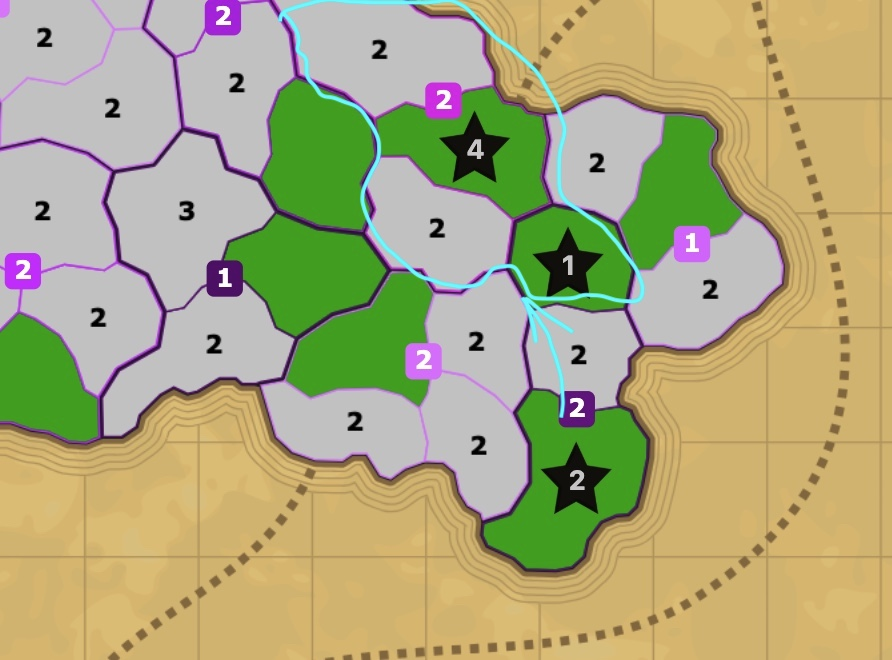
\includegraphics[width=0.7\textwidth]{Images/numenor map.jpg}
  \caption{Numenor border east}
  \label{numenor_border}
\end{figure}

Some bonuses are naturally better than others due to their position, safety, easiness of capturing and orientation of their borders. Take for example \href{https://www.warzone.com/MultiPlayer?GameID=39273878}{Tor-ture}. After an analysis of all MTL games above 1800 rating, the winrate of each bonus is given in the Figure \ref{tor-ture winrate}

\begin{figure}[H]
  \centering
  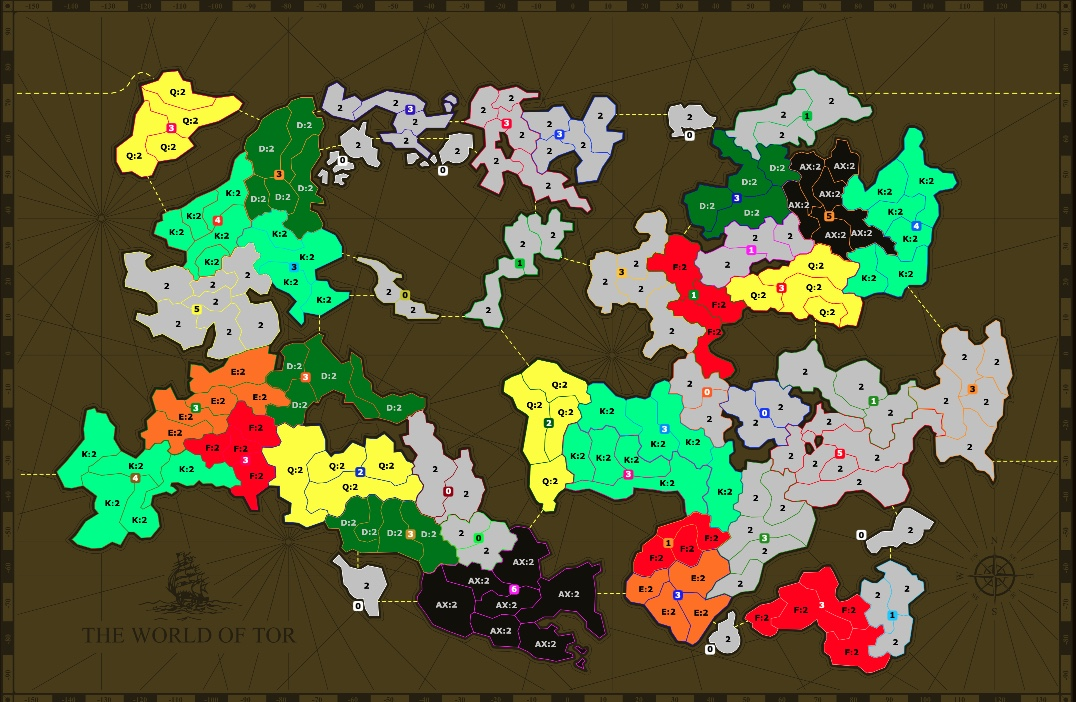
\includegraphics[width=0.95\textwidth]{Images/tor-ture1800.jpg}
  \caption{Win Rate of each bonus picked in the MTL database >1800 rating}
  \label{tor-ture winrate}
\end{figure}

The Larger black bonuses are very rarely picked under specific conditions and most of the times their opponents don't expect them. Black is win rate >60\%. Anything Green >50\%.Yellow 48-50 \% and Orange, Red below that. No coloir means either not picked or win rate well below 40 \%. Pay attention however for example on the west, and the efficient, red +3 bonus, that is very often picked as an FTB and how the light green +4 on the west holds a triple border against it. Furthermore, imagine yourself having to get 1 pick in that region. The +4 bonus can expand and complete the +3 one within 2 turns while sending useful armies towards good bonuses. The +3 bonus requires a 3-turn setup to expand either west, or east.
\\
\\
We don't generally pay attention or brute-force calculate these things, like how for example in Strat MME, from Australia you can expand in Indonesia within 2 turns, or how Indonesia only has single borders. In my opinion it's generally good to train your instinct in understanding why certain bonuses are better than others in each retrospective template and settings.